\subsection{Observer design}
\label{observer}

As it is shown in \figref{fig:statefeedback}, it is possible to find a state feedback law that gives closed-loop eigenvalues with desired dynamics and a condition that all states are measured. Even if all states are measured or measurable, the disturbances has to be taken into consideration while designing the observer. 

If a system is observable, it is possible to recover the states from measurements of the input and output of the system. The feedback law is exactly the same as in \eqref{eq:feedbacklaw} with the exception that now the disturbance is also considered and due to the separation principle it is sufficient to design the observer without the state feedback. The purpose of the observer is now to reconstruct both the system states $\mathbf{x}$ and the disturbance $d$ from the input and the output. Since the disturbance has an effect on the output, it is observable from y. Furthermore, $d$ is generally unknown, thus it is reasonable to estimate it with a help of an observer. It is important to mention that although the disturbance cannot be measured, information about its structure and periodicity are assumed to be available in this simulation. 

The system with the observer and state feedback can be represented as follows: 

%\begin{figure}[H]
%\centering
%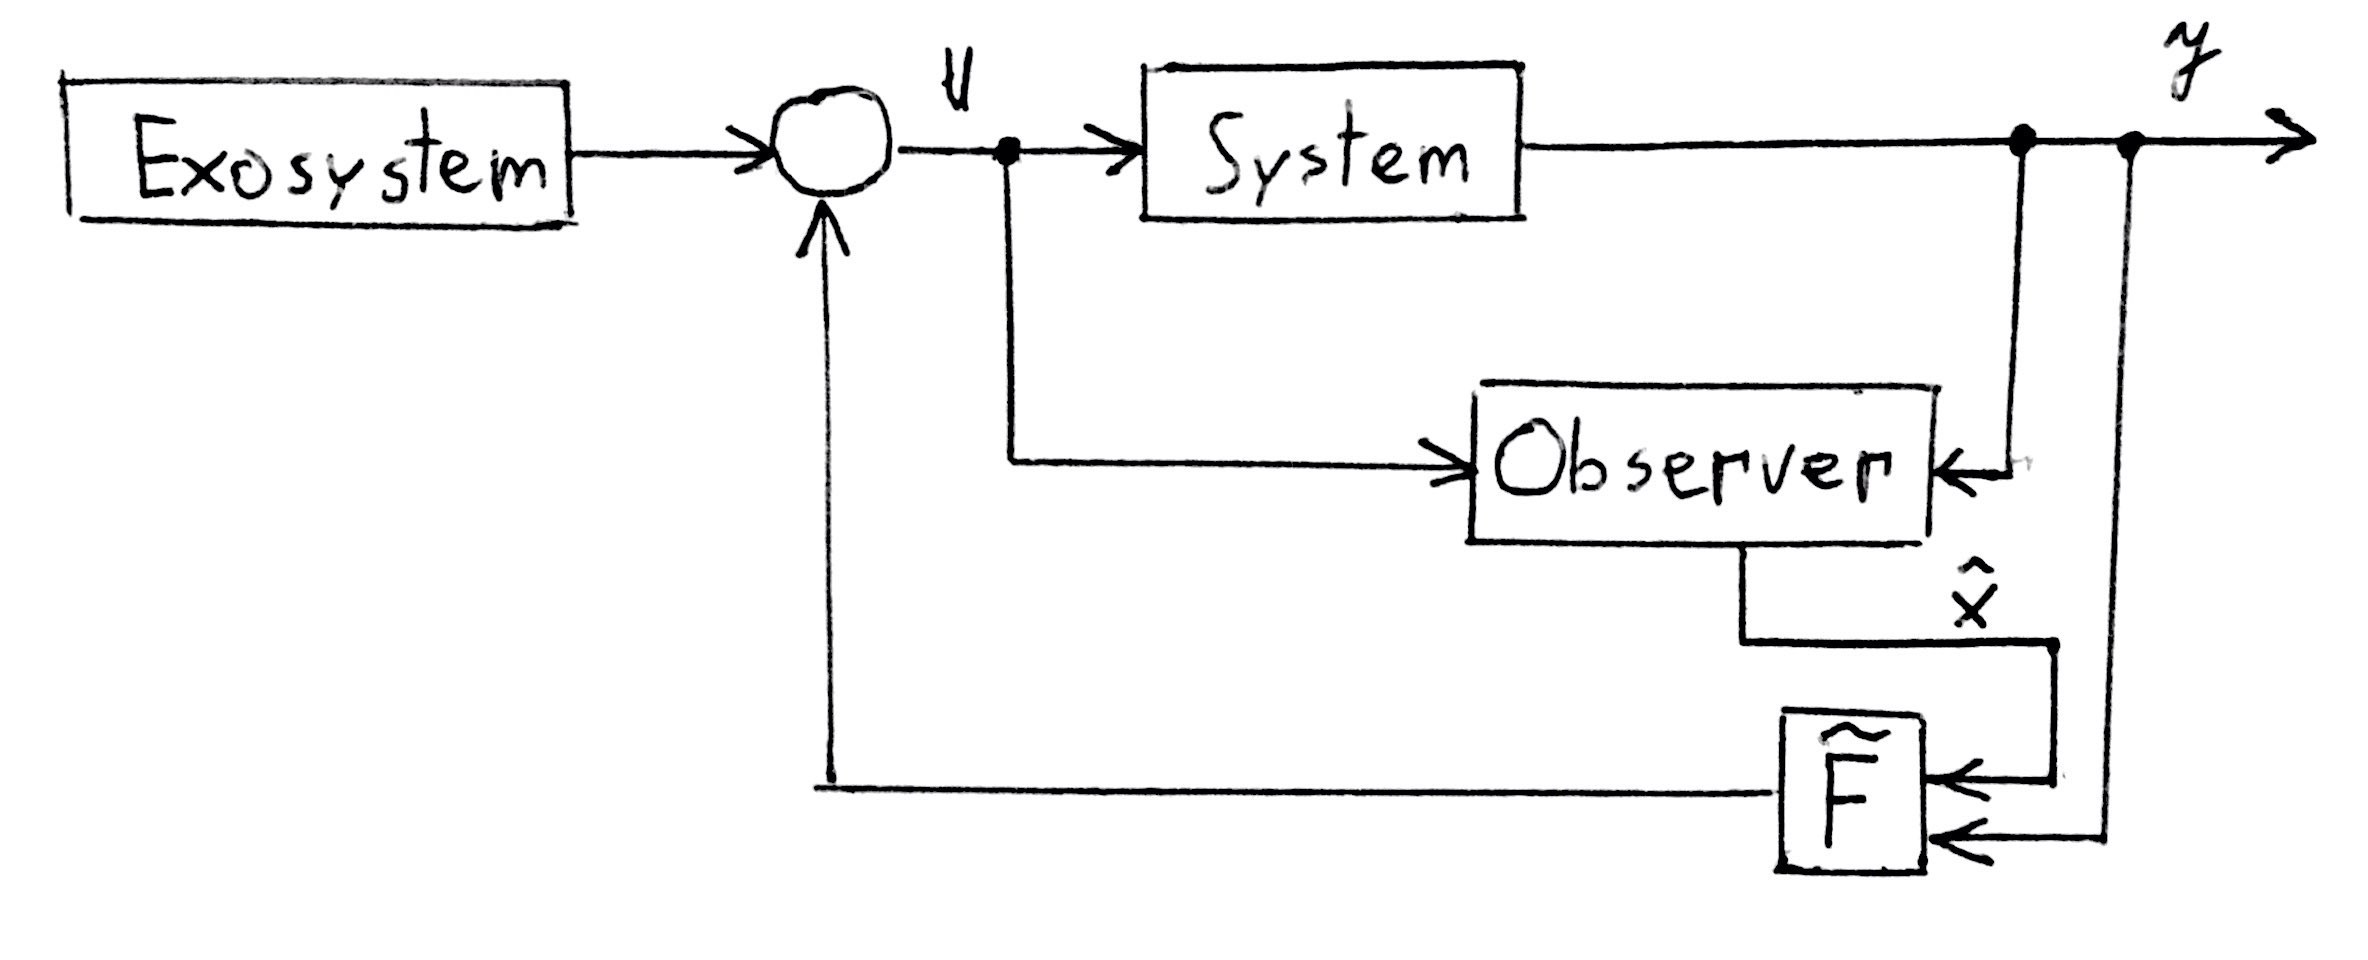
\includegraphics[width=0.65\textwidth]{rapport/billeder/observerblock}
%\caption{State feedback}
%\label{fig:observerblock}
%\end{figure}


\begin{figure}[H]
\centering
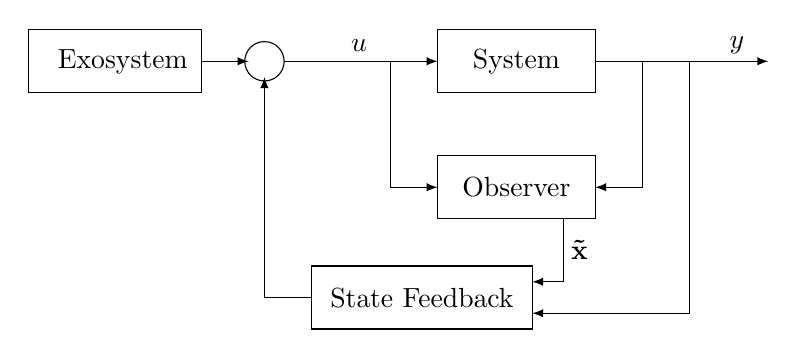
\begin{tikzpicture}


 \draw [-latex] (-1.2,2) ellipse (0.25 and 0.25);
 \node at (2,2) {\normalsize{System}};
\draw [-latex] (1,2.4) rectangle (3,1.6);
 \node at (2,0.4) {\normalsize{Observer}};


\draw [-latex] (1,0.8) rectangle (3,0);
\draw [-latex](-0.95,2) -- (1,2);
\draw [-latex](0.4,2) -- (0.4,0.4) -- (1,0.4);
\draw [-latex](3,2) -- (5.2,2);
\draw [-latex](3.6,2) -- (3.6,0.4) -- (3,0.4);

 \node at (0.8,-1) {\normalsize{State Feedback}};
 
 
\draw [-latex] (-0.6,-0.6) rectangle (2.2,-1.4);
\draw [-latex](2.6,0) -- (2.6,-0.8) -- (2.2,-0.8);
\draw [-latex](4.2,2) -- (4.2,-1.2) -- (2.2,-1.2);
\draw [-latex](-0.6,-1) -- (-1.2,-1) -- (-1.2,1.8);

\node at (-3,2) {\normalsize{Exosystem}};

\draw [-latex] (-4.2,2.4) rectangle (-2,1.6);
\draw [-latex](-2,2) -- (-1.4,2);
\node at (4.8,2.2) {\normalsize{$y$}};
\node at (0,2.2) {\normalsize{$u$}};

\node at (2.8,-0.4) {\normalsize{$\mathbf{\tilde{x}}$}};

\end{tikzpicture}
\caption{State feedback}
\label{fig:observerblock}
\end{figure}

Therefore the state-space system description becomes: 

\begin{equation}
\label{eq:ss_obs1}
\frac{d}{dt}
\begin{bmatrix}
    \mathbf{\tilde{x}} \\
    \mathbf{\tilde{x_d}} 
\end{bmatrix}
=
 \begin{bmatrix}
    \mathbf{A} & \mathbf{B}\mathbf{C_d} \\
    0 & \mathbf{A_d}
\end{bmatrix}
 \begin{bmatrix}
    \mathbf{\tilde{x}} \\
    \mathbf{\tilde{x_d}}
\end{bmatrix}
+
 \begin{bmatrix}
    \mathbf{B}  \\
    0 &  
\end{bmatrix}
    u
    +
 \begin{bmatrix}
    \mathbf{L_1}  \\
    \mathbf{L_2}  
\end{bmatrix}
 \begin{bmatrix}
    y - \mathbf{C}\mathbf{\tilde{x}}
\end{bmatrix}
\end{equation}

The modified control law:

\begin{equation}
  \label{eq:ss_obs2}
  u =  \mathbf{F} \mathbf{\tilde{x}_{combined}} 
  =
 \begin{bmatrix}
    \mathbf{F} & \mathbf{-C_d}  
\end{bmatrix}
 \begin{bmatrix}
\mathbf{\tilde{x}}  \\
\mathbf{\tilde{x_d}}
\end{bmatrix}
  \end{equation}
  
As can be seen in \eqref{eq:ss_obs2}, the feedback gain is extended in order to reproduce the disturbance and subtract it from the output. 
  
The control problem of finding the appropriate observer feedback gains simplifies to the problem of finding new locations of the closed-loop eigenvalues of the observer such as:

\begin{equation}
  \label{eq:distpoly}
    det(s\mathbf{I}-(\mathbf{\tilde{A}} + \mathbf{\tilde{L}} \mathbf{\tilde{C}}))
  \end{equation}

Since the poles of the observer should not have any effect on the system, in other words, it is undesirable to introduce new dominant poles in the system, as a rule of thumb the poles should be placed 2 to 6 times further to the left-hand side along the real axis from the poles of the state feedback. By making the observer dynamics react fast, the difference between the estimated and the real output will converge faster to zero. According to \eqref{eq:desired_poles}, the poles should be placed at: 

\begin{equation}
  \label{eq:desired_poles_observer1}
  p_{L_{3;4}} = -16 \pm j7
  \end{equation}
  
and
  
\begin{equation}
  \label{eq:desired_poles_observer2}
  p_{L_{5}} = -2 +j0
  \end{equation}
  
  \begin{equation}
  \label{eq:desired_poles_observer3}
  p_{L_{6}} = -4 +j0
  \end{equation}
  

  
  
  